\documentclass{beamer}

\DeclareMathOperator*{\argmax}{argmax}

\title{Reinforcement Learning}
\author{
    Niccolò Consigli
		\scriptsize \texttt{n.consigli@studenti.unipi.it}
		\\
		\normalsize
    Luca Seggiani
		\scriptsize \texttt{l.seggiani@studenti.unipi.it}
		\normalsize
	}
\institute{Università di Pisa}
\date{\today}

\begin{document}

\begin{frame}
	\titlepage
\end{frame}

\begin{frame}
	\frametitle{A new kind of learning}
	\begin{itemize}
		\item<1-> Supervised learning: matching features to labels
		\item<2-> Unsupervised learning: clustering data
		\item<3-> \textbf{Reinforcement learning}: learning from rewards
	\end{itemize}
\end{frame}

\begin{frame}
	\frametitle{What is reinforcement learning (RL)?}
	\begin{itemize}
		\item<1-> We give the agent \textbf{rewards} based on its performance
		\item<2-> Markov property: we can view problems as \textbf{Markov decision processes} (MDPs)
	\end{itemize}
\end{frame}

\begin{frame}
	\frametitle{A framework: Markov decision processes}
	\begin{itemize}
		\item Actions map states to states with a probability distribution
		\item Transition reward: $R(s, a, s')$
		\item Transition probability: $P(s' \, | \, s, a)$
	\end{itemize}
	\begin{center}
		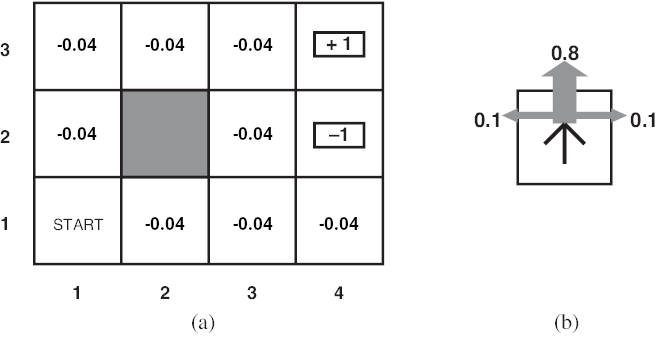
\includegraphics[scale=0.95]{figures/markov-decisional-process.png}
	\end{center}
	\pause
	\begin{block}{Bellman's equation}
		Given a discount factor $\gamma \in [0, 1]$, the utility is given by:
		$$
		U(s) = \max_{a \in A(s)} \sum_{s'} P(s' \, | \, s, a) \left[ R(s, a, s') + \gamma U(s') \right]
		$$
	\end{block}
\end{frame}

\begin{frame}
	\frametitle{Model-based reinforcement learning}
	We maintain a transition model (an \textbf{MDP}):
	\begin{itemize}
		\item Reward function: $R(s, a, s')$
		\item Probability function: $P(s' \, | \, s, a)$
		\item Utility function: U(s), maps states to \textbf{utility}
	\end{itemize}
	\pause
	Once the model is learned, we can \textbf{maximize utility}
	\begin{center}
		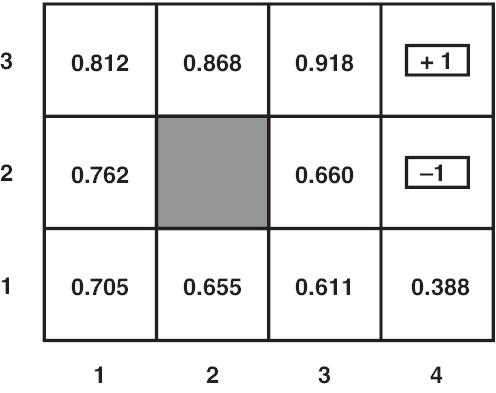
\includegraphics[scale=0.8]{figures/optimal-policy-values.png}
	\end{center}
\end{frame}

\begin{frame}
	\frametitle{Model-free reinforcement learning}
	\begin{itemize}
		\item Action-utility learning: we learn an action-utility function $Q(s, a)$ that maps \textbf{actions} to \textbf{utility}
		\item Policy search: maps \textbf{states} to \textbf{actions}, essentialy a reflex agent
	\end{itemize}
	\begin{center}
		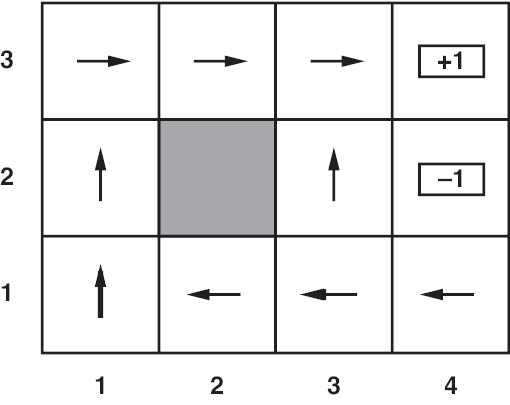
\includegraphics[scale=0.8]{figures/optimal-policy-arrows.png}
	\end{center}
\end{frame}

\begin{frame}
	\frametitle{Passive reinforcement learning}
	We can't modify the policy, but we can figure out the utilities $U(s)$
	\begin{itemize}
		\item We use \textbf{policy iteration}:
			$$
				U^\pi(s) = E\left[ \sum_{t=0}^{+\infty} \gamma^t R(s_t, \pi(s_t), s_{t+1}) \right]
			$$
	\end{itemize}
	\pause
	Three approaches for approximation:
	\begin{itemize}
		\item Direct utility estimation
		\item Adaptive dynamic programming (ADP)
		\item Temporal difference learning (TD)
	\end{itemize}
\end{frame}

\begin{frame}
	\frametitle{Direct utility estimation}
	The goal is to approximate state utility under the given policy
	\begin{itemize}
		\item Make \textbf{trials} and take the \textbf{reward-to-go} for each state
	\end{itemize}
	\pause
	\begin{block}{Example}
	We calculate utilities for $(1,2)$ given the trial:
		$$
		\scriptstyle
		(1,1) \xrightarrow[\text{Up}]{-0.4} 
		(1,2) \xrightarrow[\text{Up}]{-0.4}
		(1,3) \xrightarrow[\text{Right}]{-0.4}
		(1,2) \xrightarrow[\text{Up}]{-0.4}
		(1,3) \xrightarrow[\text{Right}]{-0.4}
		(2,3) \xrightarrow[\text{Right}]{-0.4}
		(3,3) \xrightarrow[\text{Right}]{+1}
		(4,3)
	$$
	\pause
	$$
		U(1,2) = -0.04 -0.04 -0.04 -0.04 -0.04 + 1 = 0.8
	$$
	\pause
	$$
		U(1,2)' = -0.04 -0.04 -0.04 + 1 = 0.88
	$$
	\end{block}
	\pause
	\begin{itemize}
		\item This is inefficient! We can \textbf{exploit} the Markov property 
	\end{itemize}
\end{frame}

\begin{frame}
	\frametitle{Adaptive dynamic programming}
	We can approximate the transition reward and probability functions ($P$ and $R$) and apply \textbf{simplified Bellman's equation}:
	$$
		U(s) = \sum_{s'} P(s' \, | \, s, \pi(s)) \left[ R(s, \pi(s), s') + \gamma U(s') \right]
	$$
	When the policy is fixed, this gives a \textbf{linear equation}
	\pause
	\begin{itemize}
		\item Calculating $P$ and $R$ is easy when the environment is \textbf{fully observable} 
	\end{itemize}
\end{frame}

\begin{frame}
	\frametitle{Temporal difference learning}
	Still taking trials, but we \textbf{update} the utility to match frequently observed transitions
	\begin{itemize}
		\item We don't need a model!
	\end{itemize}
	\pause
	\begin{block}{Example}
	We calculate utilities for transiton $(1,3) \rightarrow (2,3)$ given the trial:
		$$
		\scriptstyle
		(1,1) \xrightarrow[\text{Up}]{-0.4} 
		(1,2) \xrightarrow[\text{Up}]{-0.4}
		(1,3) \xrightarrow[\text{Right}]{-0.4}
		(2,3) \xrightarrow[\text{Right}]{-0.4}
		(3,3) \xrightarrow[\text{Right}]{-0.04}
		(3,2) \xrightarrow[\text{Up}]{-0.04}
		(3,3) \xrightarrow[\text{Right}]{+1}
		(4,3)	
	$$
	and the previous utility estimates: $U^\pi(1,3) = 0.88, \ U^\pi(2,3) = 0.96$
	\pause
	$$
		U^\pi (1, 3)' = -0.04 + U^\pi (2,3)
	$$
	\begin{itemize}
		\item This gives $U^\pi(1,3)' = 0.92$, which means $0.88$ might be a low estimate
	\end{itemize}	
	\end{block}
\end{frame}

\begin{frame}
	\frametitle{Temporal difference learning (continued)}
	We want to match $U^\pi$ to $U^\pi'$ with learning rate $\alpha$:
	$$
		U^\pi(1,3) \leftarrow U^\pi(1,3) + \alpha \left[ U^\pi(1,3)' - U^\pi(1,3) \right]
	$$
	Which generalizes to:
	$$
	U^\pi(s) \leftarrow U^\pi(s) + \alpha \left[ R(s, \pi(s), s') + \gamma U^\pi (s') - U^\pi (s) \right]
	$$
	\begin{itemize}
		\item From TD's point of view, ADP is TD with \textit{simulated experiences}
	\end{itemize}
\end{frame}

\begin{frame}
	\frametitle{Active reinforcement learning}
	Utility functions give the best (expected) policy
	
	We can decide to improve utility (\textbf{explore}) or keep maximizing utility (\textbf{exploit})
	\begin{itemize}
		\item This is a \textbf{multi-armed bandit problem} (set of Markov reward processes)
	\end{itemize}
	\pause
	\begin{block}{Example}
		Duolingo's recurring notifications use a bandit problem solver:
		\begin{columns}
		\begin{column}{0.4\textwidth}
			\begin{center}
				
\includegraphics[scale=0.24]{figures/duolingo_notifications.png}
			\end{center}
		\end{column}
		\begin{column}{0.6\textwidth} %
			\begin{center}
				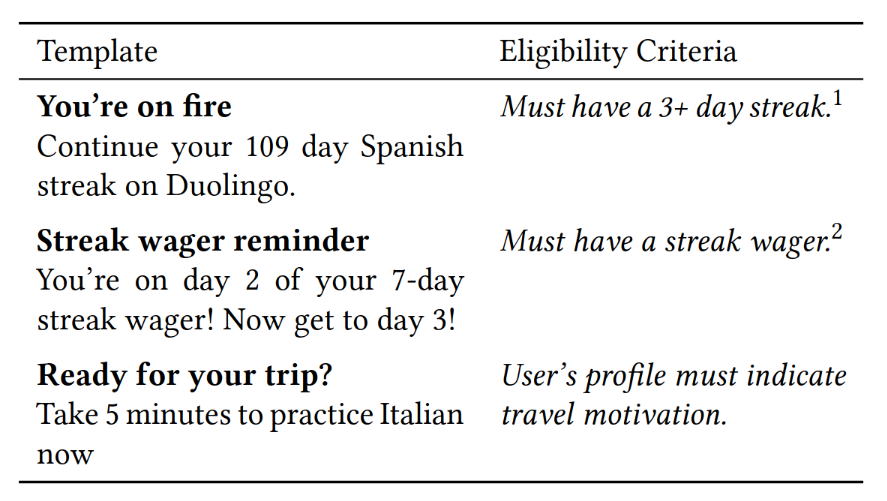
\includegraphics[scale=0.25]{figures/duolingo_eligibility.png}
			\end{center}
		\end{column}
		\end{columns}
	\end{block}
\end{frame}

\begin{frame}
	\frametitle{Greedy in the limit of infinite exploration (GLIE)}
	A greedy algorithm could ignore higher utility actions.
	We need a GLIE algorithm:
	\begin{itemize}
		\item Each eaction in a each state is tried an unbounded amount of times
		\item In the limit ($\rightarrow \infty$) the algorithm becomes truly greedy
	\end{itemize}
	\pause 
	We can try different approaches:
	\begin{itemize}
		\item<1-> Random sampling
		\item<2-> Minimum trials
	\end{itemize}
\end{frame}

\begin{frame}
	\frametitle{Random sampling}
	At step $t$, do the following:
	\begin{itemize}
		\item Choose a random action with probability $\frac{1}{t}$
		\item Otherwise, follow the greedy policy
	\end{itemize}
	This \textbf{does} eventually converge, but can be slow: a better approach would use some heuristic on state utility
\end{frame}

\begin{frame}
	\frametitle{Minimum trials}
	Have an \textbf{optimistic estimate} of utility ($U^+(s)$):
	$$
	U^+(s) \leftarrow \max_a f \left( \sum_{s'} P(s' \, | \, s, a) \left[ R(s, a, s') + \gamma U^+(s') \right], N(s, a) \right)	
	$$
	\begin{itemize}
		\item $N(s,a)$ is the number of times action $a$ was tried from state $s$
		\item $f$ is defined as:
			$$
				f(u, n) = 
				\begin{cases}
					R^+, \quad n < N_e \\ 
					u, \quad \ \ \, n \geq N_e
				\end{cases}
			$$
			Here, $R^+$ is an optimistic utility for actions tried less than $N_e$ times
	\end{itemize}
	Basically, we are estabilishing an optimistic \textbf{prior} that assigns higher utilities to actions tried less than $N_e$ times
\end{frame}

\begin{frame}
	\frametitle{Safe exploration}
	In the real world, we have to look out for:
	\begin{itemize}
		\item Large negative rewards
		\item Absorbing states 
		\item Irreversible actions 
	\end{itemize}
	Neither the greedy nor the exploratory approach are optimal!
	\pause
	Three ways to solve the problem:
	\begin{itemize}
		\item Bayesian reinforcement learning
		\item Partially Observable MDPs
		\item Robust control theory approach
	\end{itemize}
\end{frame}

\begin{frame}
	\frametitle{Bayesian reinforcement learning}
	We take a probabilistic approach, starting with a \textbf{prior} probability $P(h)$ on $h$ hypotheses about what the model \textbf{is}: the policy is then given by the posterior $P(h \, | \, e)$:
	$$
		\pi^* = \argmax_\pi \sum_h P(h \, | \, e) U_h^\pi
	$$
	\pause
	\begin{itemize}
		\item Note that this approach assumes that the prior contains good estimates of reality
		\item We can turn this into an exploration POMDP where belief states are distributions over models
	\end{itemize}
\end{frame}

\begin{frame}
	\frametitle{The robust control theory approach}
	We define a set of models $\mathcal{H}$, and always take the policy that maximizes utility in the \textbf{worst case} over $\mathcal{H}$:
	$$
		\pi^* = \argmax_\pi \min_h U_h^\pi
	$$
	\pause
	\begin{itemize}
		\item This is closely tied to bayesian reinforcement learning: the set $\mathcal{H}$ is the set of models that exceed some likelihood threshold on $P(h \, | \, e)$
		\item In both cases we assume the models to be good estimates of reality
	\end{itemize}
\end{frame}

\begin{frame}
	\frametitle{Temporal difference Q-learning}
	\begin{itemize}
		\item<1-> With TD learning, we estimated the utility under a given policy
		\item<2-> Now we can estimate the action-utility functions in order to improve the policy
	\end{itemize}
	\pause
	\pause
	We substitute $Q(s,a)$ into Bellman's equation:
	$$
		Q(s, a) = \sum_{s'} P(s' | s, a) \left[ R(s, a, s') + \gamma \max_{a'} Q(s', a') \right]
	$$
	Now we can derive an update:
	$$
	Q(s, a) \leftarrow Q(s, a) + \alpha \left[ R(s, a, s') + \gamma \max_{a'} Q(s', a') - Q(s, a) \right]
	$$
\end{frame}

\begin{frame}
	\frametitle{SARSA learning}
	SARSA is a variation of TD Q-learning: instead of assuming the best possible action under known action-utility functions to be taken (\textbf{off-policy}), we wait for the model to actually execute actions (\textbf{on-policy})
	\begin{itemize}
		\item We act after $s, a, r, s', a'$ quintuplets
	\end{itemize}
	The update is given by:
	$$
		Q(s, a) \leftarrow Q(s, a) + \alpha \left[ R(s, a, s') + \gamma Q(s', a') - Q(s, a) \right]
	$$
	\pause
	TD and SARSA are subtly different:
	\begin{itemize}
		\item TD learning asks: "What does this action give if i stop using my policy, and take the best action (according to my estimates) from there onwards?"
		\item SARSA asks: "What did I get when i followed my policy and took this action?" 
	\end{itemize}
\end{frame}

\end{document}
